%\documentclass[
  bibliography=totoc,     % Literatur im Inhaltsverzeichnis
  captions=tableheading,  % Tabellenüberschriften
  titlepage=firstiscover, % Titelseite ist Deckblatt
]{scrartcl}

% Paket float verbessern
\usepackage{scrhack}

% Warnung, falls nochmal kompiliert werden muss
\usepackage[aux]{rerunfilecheck}

% unverzichtbare Mathe-Befehle
\usepackage{amsmath}
% viele Mathe-Symbole
\usepackage{amssymb}
% Erweiterungen für amsmath
\usepackage{mathtools}

% Fonteinstellungen
\usepackage{fontspec}
% Latin Modern Fonts werden automatisch geladen
% Alternativ zum Beispiel:
%\setromanfont{Libertinus Serif}
%\setsansfont{Libertinus Sans}
%\setmonofont{Libertinus Mono}

% Wenn man andere Schriftarten gesetzt hat,
% sollte man das Seiten-Layout neu berechnen lassen
\recalctypearea{}

% deutsche Spracheinstellungen
\usepackage[ngerman]{babel}


\usepackage[
  math-style=ISO,    % ┐
  bold-style=ISO,    % │
  sans-style=italic, % │ ISO-Standard folgen
  nabla=upright,     % │
  partial=upright,   % │
  mathrm=sym,        % ┘
  warnings-off={           % ┐
    mathtools-colon,       % │ unnötige Warnungen ausschalten
    mathtools-overbracket, % │
  },                       % ┘
]{unicode-math}

% traditionelle Fonts für Mathematik
\setmathfont{Latin Modern Math}
% Alternativ zum Beispiel:
%\setmathfont{Libertinus Math}

\setmathfont{XITS Math}[range={scr, bfscr}]
\setmathfont{XITS Math}[range={cal, bfcal}, StylisticSet=1]

% Zahlen und Einheiten
\usepackage[
  locale=DE,                   % deutsche Einstellungen
  separate-uncertainty=true,   % immer Unsicherheit mit \pm
  per-mode=symbol-or-fraction, % / in inline math, fraction in display math
]{siunitx}

% chemische Formeln
\usepackage[
  version=4,
  math-greek=default, % ┐ mit unicode-math zusammenarbeiten
  text-greek=default, % ┘
]{mhchem}

% richtige Anführungszeichen
\usepackage[autostyle]{csquotes}

% schöne Brüche im Text
\usepackage{xfrac}

% Standardplatzierung für Floats einstellen
\usepackage{float}
\floatplacement{figure}{htbp}
\floatplacement{table}{htbp}

% Floats innerhalb einer Section halten
\usepackage[
  section, % Floats innerhalb der Section halten
  below,   % unterhalb der Section aber auf der selben Seite ist ok
]{placeins}

% Seite drehen für breite Tabellen: landscape Umgebung
\usepackage{pdflscape}

% Captions schöner machen.
\usepackage[
  labelfont=bf,        % Tabelle x: Abbildung y: ist jetzt fett
  font=small,          % Schrift etwas kleiner als Dokument
  width=0.9\textwidth, % maximale Breite einer Caption schmaler
]{caption}
% subfigure, subtable, subref
\usepackage{subcaption}

% Grafiken können eingebunden werden
\usepackage{graphicx}

% schöne Tabellen
\usepackage{tabularray}
\UseTblrLibrary{booktabs, siunitx}

% Verbesserungen am Schriftbild
\usepackage{microtype}

% Literaturverzeichnis
\usepackage[
  backend=biber,
]{biblatex}
% Quellendatenbank
\addbibresource{lit.bib}
\addbibresource{programme.bib}

% Hyperlinks im Dokument
\usepackage[
  german,
  unicode,        % Unicode in PDF-Attributen erlauben
  pdfusetitle,    % Titel, Autoren und Datum als PDF-Attribute
  pdfcreator={},  % ┐ PDF-Attribute säubern
  pdfproducer={}, % ┘
]{hyperref}
% erweiterte Bookmarks im PDF
\usepackage{bookmark}

% Trennung von Wörtern mit Strichen
\usepackage[shortcuts]{extdash}

\author{%
  Vincent Wirsdörfer\\%
  \href{mailto:vincent.wirsdoerfer@udo.edu}{authorA@udo.edu}%
  \and%
  Joris Daus\\%
  \href{mailto:joris.daus@udo.edu}{authorB@udo.edu}%
}
\publishers{TU Dortmund – Fakultät Physik}


%\begin{document}

\section{Diskussion}
\label{sec:Diskussion}

\noindent Prinzipiell sind die gemessenen Ergebnisse des Versuchs zum Geiger-Müller-Zähler als positiv zu bewerten. Im Wesentlichen 
gilt es sowohl die Steigung des GM-Plateaus, als auch die Totzeit des Detektors auf zwei verschiedene Art und Weisen zu bestimmen. 
Im Optimalfall sind die jeweiligen Werte der Methoden selbstverständlich identisch. Aufgrund systematischer Fehlereinflüsse
sind Differenzen jedoch unvermeidbar. Diese sollen im Folgenden näher betrachtet werden.\\

\noindent Wie dem vorherigen Kapitel \ref{sec:Auswertung} zu entnehmen ist, wird die Steigung einerseits durch eine lineare 
Regression und andererseits durch die Formel \eqref{eqn:mPlateau} berechnet. Mittels dieser Methoden werden die folgenden 
Werte bestimmt:

\begin{align*}
    a_\text{Reg.} &= \qty{0.032\pm0.011}{\per \volt \per \second} \cdot 100\% / \qty{100}{\volt}\\
    a_\text{Form.} &= \qty{0.038\pm0.001}{\per \volt \per \second} \cdot 100\% / \qty{120}{\volt}
\end{align*}

\noindent Die Mittelwerte beider Messergebnisse unterscheiden sich erst in der dritten Nachkommastelle, was auf eine erfolgreiche 
und gelungene Untersuchung des Plateaus schließen lässt. Zusätzlich soll die Totzeit, also das Zeitintervall der Inaktivität des 
Geiger-Müller-Zählers untersucht werden. Hierzu wird die auf dem Oszilloskop erkennbare Graphik und die Formel \eqref{eqn:Totzeit}
verwendet.

\begin{align*}
    \tau_\text{Osz.} &= \qty{260\pm5}{\micro \second}\\
    \tau_\text{Form.} &= \qty{112.2\pm1.7}{\micro \second}
\end{align*}

\noindent Diese Werte weichen um den Faktor 2 voneinander ab. Dieses Ergebnis kann auf folgende Gründe zurückgeführt werden. \\

\noindent Aufgrund der Tatsache, dass Großteile des Experiments bereits vorbereitet sind und sich der studentische Arbeitsverlauf 
essenziell auf die Bedienung der vorhandenen Geräte beschränkt, ist eine direkte Auflistung systematischer Fehlerquellen 
erschwert. Nichtsdestotrotz können auch beim Ablesen von analogen und digitalen Geräten Fehler passieren. So zum Beispiel 
zeigt die Abbildung \ref{fig:Oszilloskop}, wie komplex die Erkennung der tatsächlichen Totzeit mit dem Oszilloskop wegen der 
Verzerrtheit der Graphik ist. Also der Fakt, dass mehrere Kurven übereinander liegen. Dies könnte somit einen direkten Einfluss auf 
die Abweichung der bestimmten Totzeiten haben.
Ferner ist der Parallaxenfehler beim Ablesen der Stromstärken nicht zu vernachlässigen, welcher durch die Schwingung der Messnadel
verstärkt wird. Ein weiterer Bereich des Fehlerspektrums wird durch die Trägheit der Instrumente wie zum Beispiel des Vorverstärkers 
oder des Zählers abgedeckt. Somit können tatsächliche, durch ionisierende Strahlung verursachte, Impulse nicht gemessen werden, 
was den Verlauf der Kennlinie und daher auch die Steigung der Regressionsgerade maßgeblich beeinflusst. Außerdem können die Zählraten 
bei Überschreiten des Maximums nicht genau abgelesen werden, was die totale Zählrate verfälscht.
Die Akkumulation dieses Fehlerspektrums sind dementsprechend potentielle Gründe für die abweichenden Ergebnisse der jeweiligen Methoden.   
 
\section{Anhang}

\begin{figure}[H]
    \centering 
    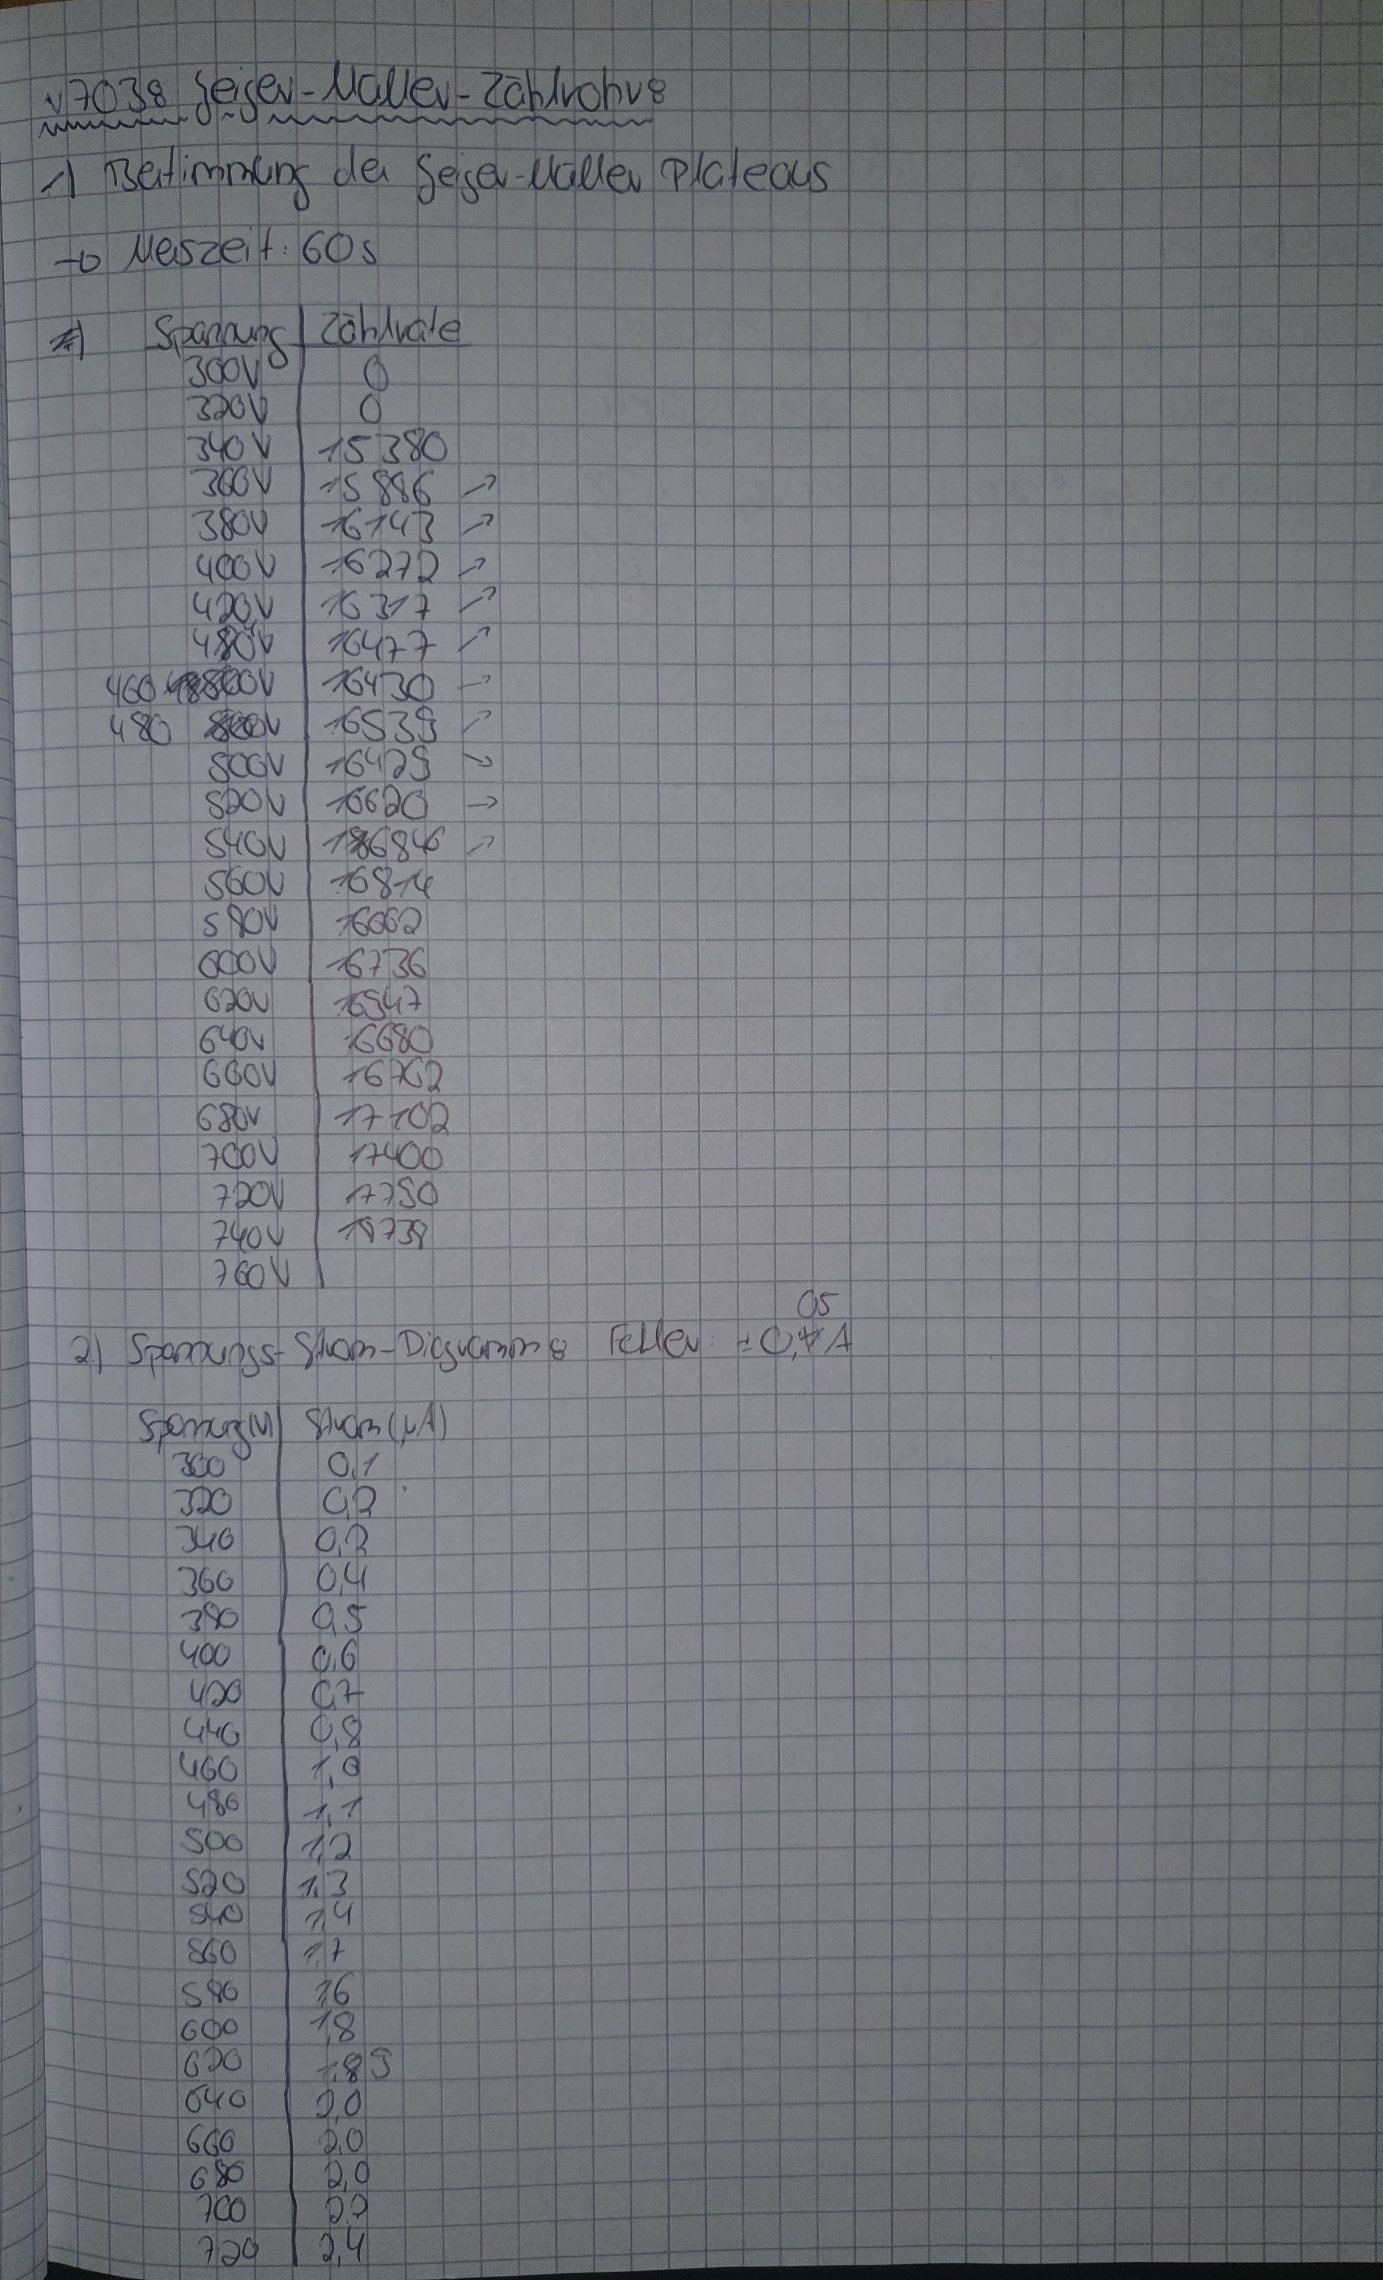
\includegraphics[width=0.9\textwidth]{content/v703_Laborbuch1.jpg}
\end{figure}

\begin{figure}[H]
    \centering 
    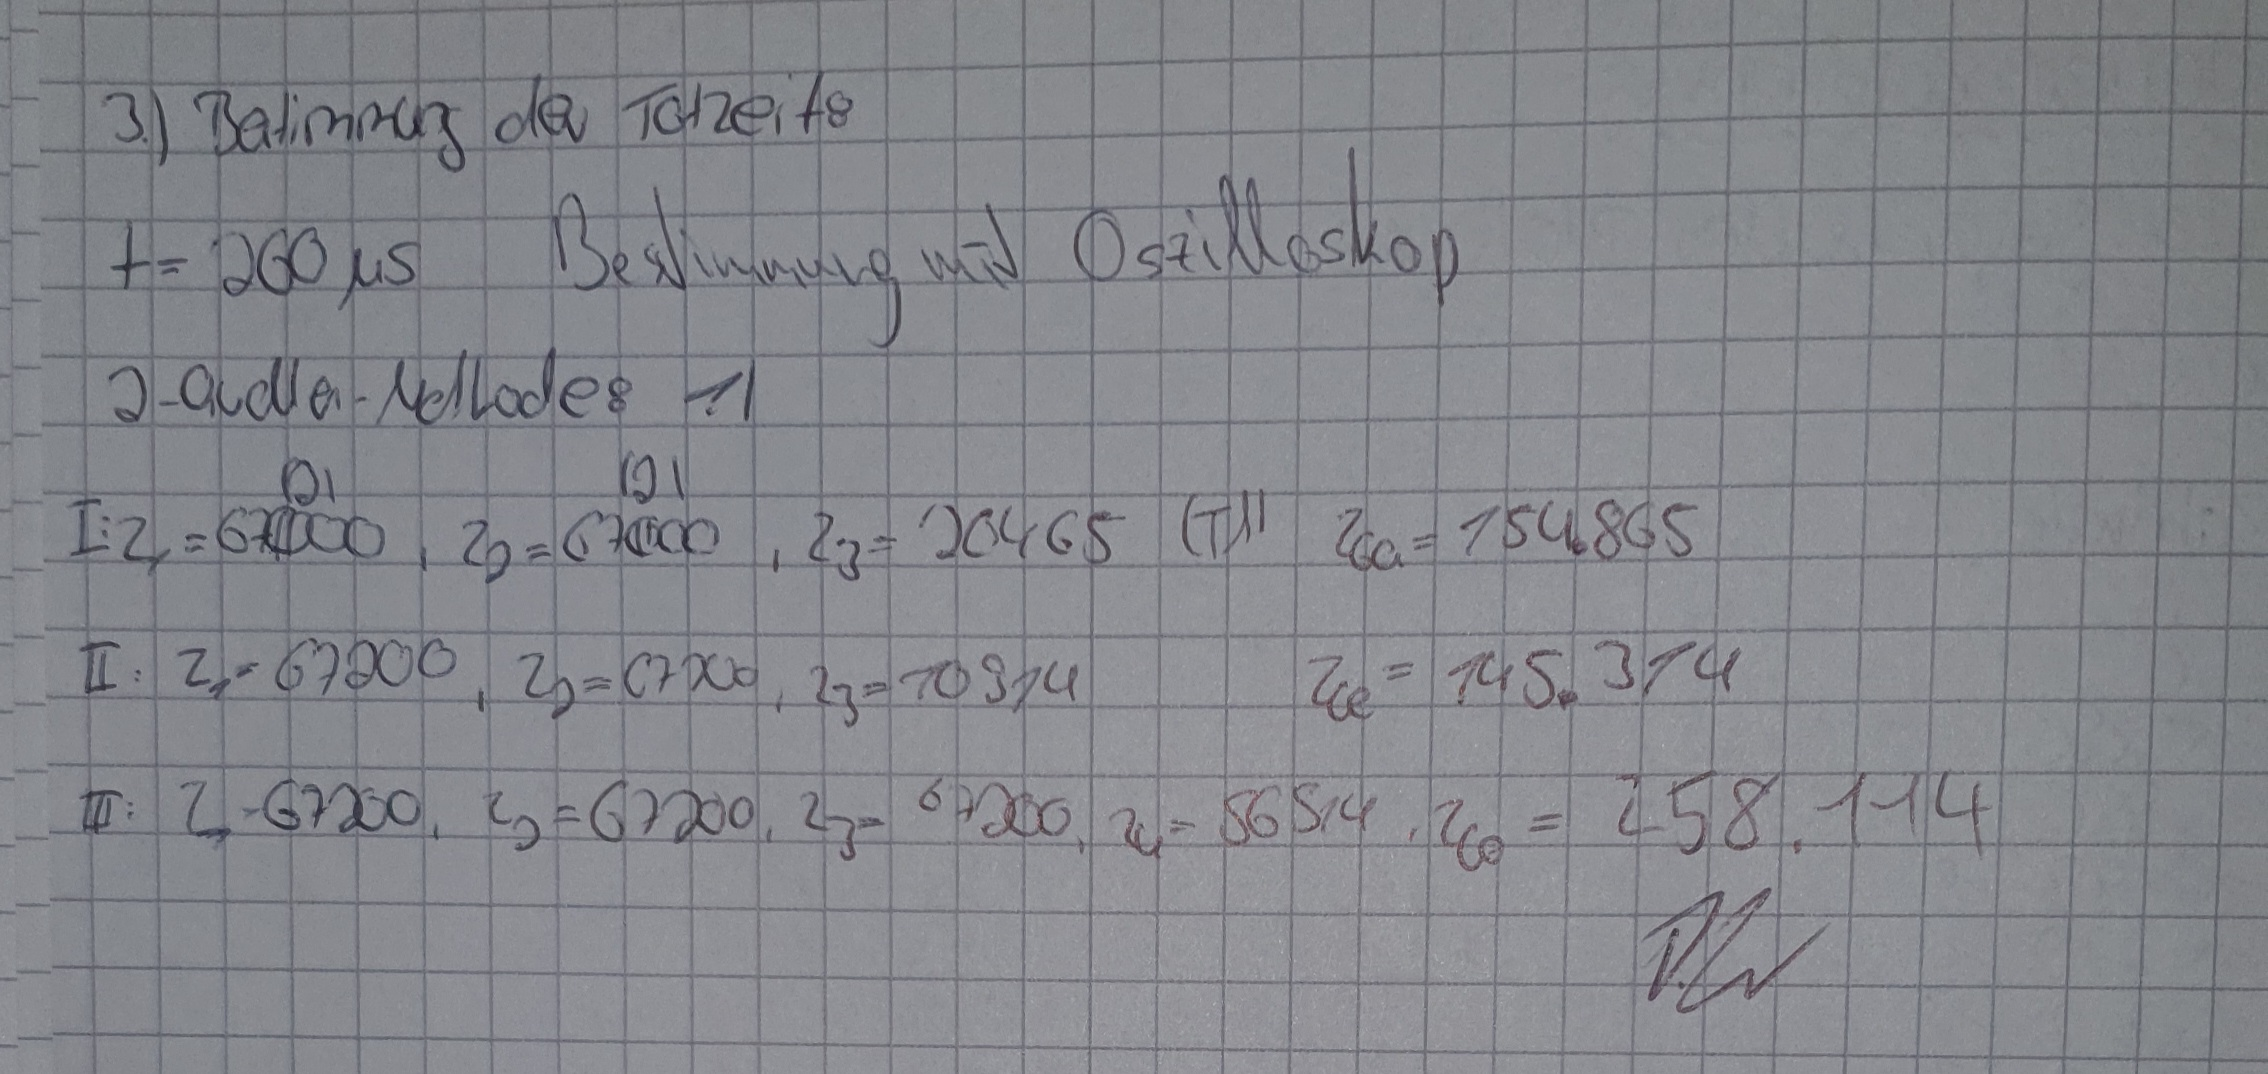
\includegraphics[width=0.9\textwidth]{content/v703_Laborbuch2.jpg}
\end{figure}

%\end{document}
